\chapter{概率}
根据作者估计,你看完这本书的概率不足10\%。根据作者再估计,你在看完这本书并且理解里面的每一个字的情况下,A-Level考到$A^*$的概率达到90\%。请问,这当中那些出现了条件概率,出现了哪些事件,读书与考$A^*$是独立事件吗?

\section*{学习目标}
\begin{todolist}
	\item 理解概率论当中的基本定义,包括\gls{event},\gls{independ},\gls{mutualexclusive},\gls{opposite}以及标记手段
	\item 通过\textbf{枚举}的手段计算事件的概率
	\item 利用韦恩图表示两个事件之间的关系
	\item 理解独立事件的判断
	\item 理解互斥事件的判断
	\item 理解概率相乘或者相加的关系
	\item 利用排列和组合求算概率
	\item 利用tree diagram求算联合事件的概率
	\item 掌握\gls{bayes}公式,并求算\gls{condi}
\end{todolist}

\clearpage

\section{一些基本概念}
在做计算前,先了解概率论的一些基本定义

\subsection*{随机事件以及概率}
在概率论当中我们研究的是一个随机事件,是执行一个实验,产生所有可能结果。比如扔一个骰子或者硬币就是一个随机实验,扔出6朝上或者人头朝上就是这次随机实验的随机事件。这种例子可能已经看匿了。

那换一个难但是更加有趣的例子:
在地铁上airdrop下面图像就是一个随机实验,对方接收就是一个事件。对方不接收也是一种随机事件。
\begin{figure}[H]
\centering

\includegraphics[width=0.3\textwidth]{airdrop}
\caption{版权如水印}
\end{figure}
猜测一下,这张图片被接收的概率

现在,如果airdrop的图像是下面的这一张
\begin{figure}[H]
\centering

\includegraphics[width=0.3\textwidth]{airdrop-rangzuo}
\caption{版权如水印}
\end{figure}
那么,这个事件的概率会上升还是会下降?
感兴趣的同学可以在地铁上试试,但是不要早上或者晚上,因为这样做,早晚是要被揍的。

因此,一般可以用文字来描述某个事件。用大写字母$A$表示。计作$A$:对方接收airdrop的图片。则$P(A)$表示这个概率。

笔者就曾经因为使用高圆圆的头像,而在地铁中收到airdrop的微信二维码截图。呵呵

\subsection*{对立事件}
对立事件是指两个事件互相排斥,且两个事件当中如果一个没有发生,另外一个必定要发生。$A$事件的对立事件可以计作$\bar{A}$ 或者说$A'$。比如$A:$李建钢是个女生。那么$A':$李建刚是个男生
\begin{figure}[H]
\centering

\includegraphics[width=0.4\textwidth]{lijiangang}
\caption{大侠卢小鱼当中的李建钢}
\end{figure}

所以有
\[
	P(A)+P(A')=1
\]
有的时候,研究某个事件的对立事件可能会更加简单。


\subsection*{联合事件}
\gls{joint}是指两个随机事件同时发生,作为一个整体,其概率的标记手段有:$P(AB)$,$P(A \text{ and }B)$或者是$P(A\cap B)$。如果使用韦恩图来表示的话,就是A事件和B事件重叠的部分。如下图所示:
\begin{figure}[H]
\centering
\includegraphics[width=0.4\textwidth]{venn}
\label{fig:venn}
\caption{利用韦恩图表示联合事件的概率}
\end{figure}

\subsection*{独立事件}
如果两个或者多个事件之间互不干扰,一个事件的发生与否并不会影响到另外一个事件的发生与否。就称这样的事件是独立事件。比如$A$:airdrop被别人接收;$B$:今天下雨这两个事件并不会有任何影响。别人接不接收了airdrop的图片,对下雨的概率没有任何影响。反之亦然,今天下不下雨都不会影响别人接收不接收airdrop的图片。那么很明显,如果$A$ $B$构成的联合事件的概率就得运用\textbf{乘法原理},直接用这两个概率的乘积即可。即:
\[
	P(AB) = P(A) \cdot P(B)
\]
这个关系也可以用来反向证明,$A$ $B$两个事件是互相独立的

\begin{ExampleBox}
In a group of $30$ adults, $25$ are right-handed and $8$ wear spectacles. The number who are right-handed and do not wear spectacles is $19$. The following table shows the numbers of the adults in each category.
\begin{table}[H]
\centering
\begin{tabular}{|l|c|c|c|}
\hline
             & Wears spectacles & Does not wear spectacles & Total \\ \hline
Right-Handed & 6                & 19                       & 25    \\ \hline
Left-Handed  & 2                & 3                        & 5     \\ \hline
Total        & 8                & 16                       & 30    \\ \hline
\end{tabular}
\end{table}

An adult is chosen at random from the group. Event $X$ is ‘the adult chosen is right-handed’; event $Y$ is ‘the adult chosen wears spectacles’.

Determine whether $X$ and $Y$ are independent events, justifying your answer.


\makebox{}\hfill Adapted from 2016 summer qp63 Q1

\tcblower
根据表格$P(X) = \frac{25}{30}$, $P(Y) = \frac{8}{30}$

$X\cap Y$代表着the adult chosen is right-handed and wears spectacles.

概率为$P(X\cap Y) = \frac{6}{30}\neq P(X) \cdot P(Y)$
因此\textbf{不是}独立事件。
\end{ExampleBox}

\subsection*{互斥事件}
如果两个事件不能同时发生,也就是$P(A\cap B)=0$,就称这两个事件是互斥事件。比如,忘记充电导致手机没电 $\cap$ 在地铁上用手机传airdrop被别人接收。

\subsection*{$P(A\cup B)$}
表示$A$ or $B$事件\textbf{至少发生一个}。当然,根据\ref{fig:venn},很简单就可以推导出:
\[
	P(A\cup B) = P(A)+P(B)-P(A \cap B)
\]

如果已知$A$ or $B$事件是互斥事件,那么 $P(A\cup B) = P(A)+P(B)$
\clearpage


\section{求算概率}
ball ball各位看一下这一条优美的概率题:\href{https://www.bilibili.com/video/BV17W411a74F?share_source=copy_web}{如何优雅地解答最难数学竞赛的压轴题}。尤其是该视频从5min57s开始。将数学思维的优美和巧妙直接呈现在你面前。

\subsection*{乘法原理}
如果实现一个事件$A$,有很多\textbf{子步骤}$A_1,\ A_2 \ldots$。并且这些步骤之间都是\textbf{互相独立}的。那么,我们就可以利用\emph{乘法原理}。把这些步骤的概率相乘得到事件$A$的概率。公式如下:
\[
	P(A)=P(A_1)\cdot P(A_2) \cdot \ldots 	
\]

比如,要想在地铁上使别人接收airdrop图片计作事件$A$。首先$A_1:$手机要有电, $A_2:$对方打开蓝牙和airdrop开关;$A_3:$对方点击接收
因此这三个概率之积才能作为``在地铁上图片被人接收的概率''

\subsection*{加法原理}
如果实现一个事件$A$,有很多\textbf{互相替代步骤}$A_1,\ A_2 \ldots$。并且这些步骤之间都是\textbf{互相排斥}的。那么,我们就可以利用\emph{加法原理}。把这些步骤的概率相加得到事件$A$的概率。公式如下:
\[
	P(A)=P(A_1) + P(A_2) \cdot \ldots 	
\]

比如,要想在地铁上用\emph{一个设备}使别人接收airdrop图片计作事件$A$。那么$A_1:$用iPhone让别人接收图片, $A_2:$用iPad让别人接收图片,$A_3:$用Macbook让别人接收图片.$A_4:$用iMac让别人接收图片。
\begin{figure}[H]
\centering
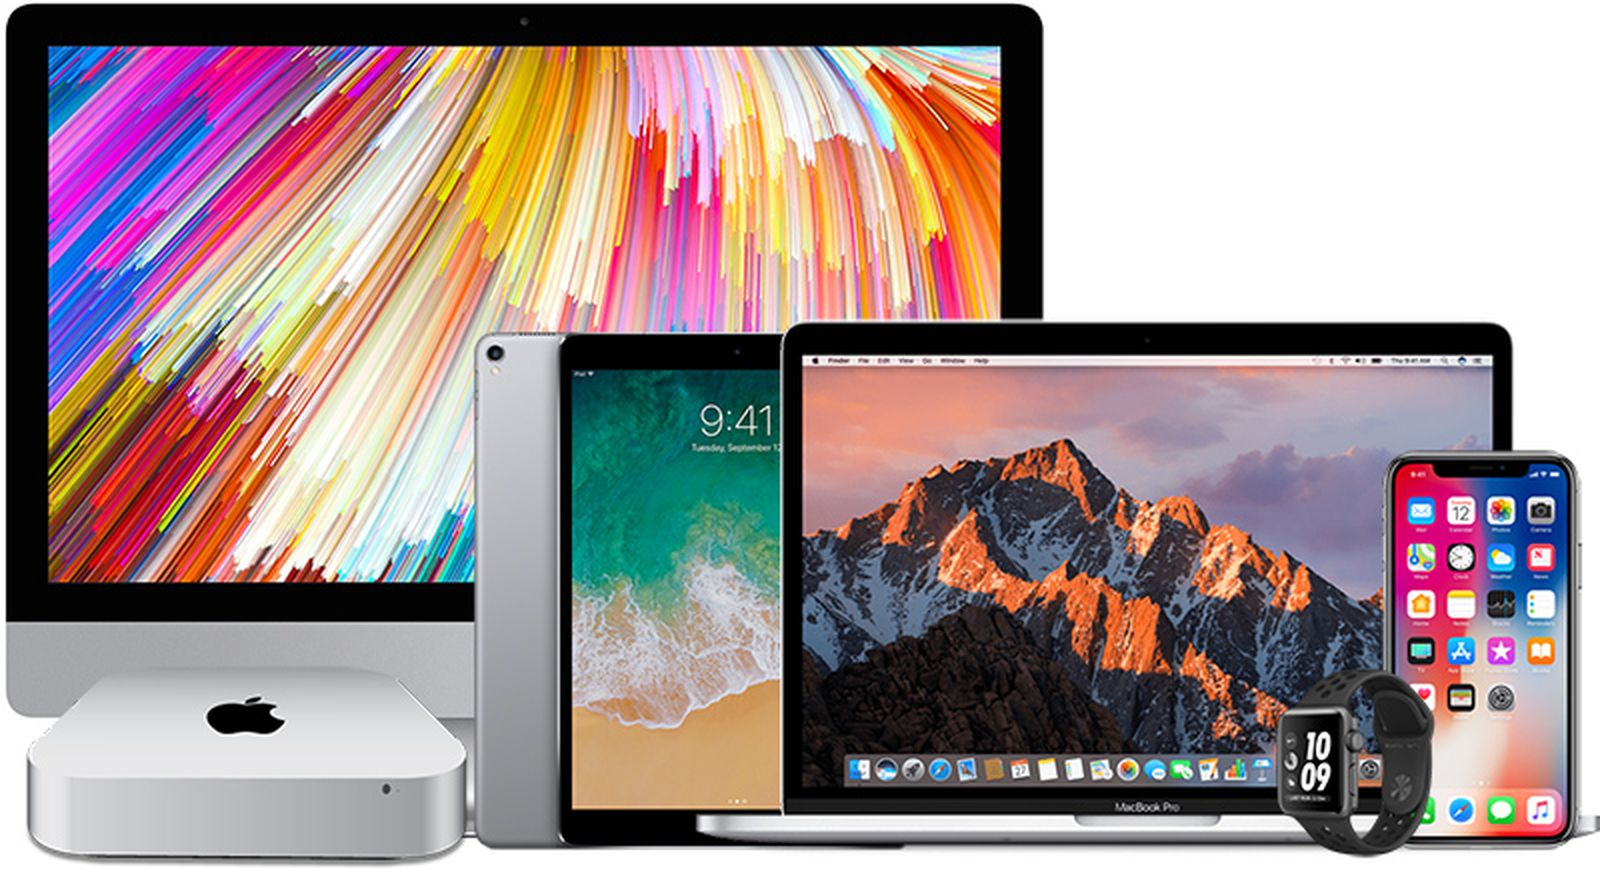
\includegraphics[width=0.8\textwidth]{appleproduct}
\caption{苹果的很多产品都具有airdrop功能}
\end{figure}


因此将这些概率相加就会得到$P(A)$。当然,由于iMac在地铁上没有电源可用,因此$P(A_3)=0$。可以省略。怎么样,是不是非常严谨!(btw,苹果公关请支付广告费用。)

在上面的两种情况中,我们可以做出如下的总结:
\begin{SummBox}
1. 如果两个事件必须同时发生才能达到目标结果(and),并且两个事件之间是互相\textbf{独立}的。则需要采用乘法原理;

2. 如果两个事件当中只需要其中一个发生就能达到目标结果(or),并且两个事件之间互相\textbf{排斥}的。则使用乘法原理;
\end{SummBox}


\subsection*{条件概率}
条件概率也被称之为后验概率,是在某个事件$B$发生的情况下,再求算$A$事件发生的概率。计作$P(A|B)$
\[
	P(A|B) = \frac{P(A\cap B)}{P(B)}
\]
\begin{SummBox}
记忆这个公式非常简单,只需要明白${A|B}$在$|$符号右边的是已经发生的事情,是确定性事件,因此出现在计算的\textbf{分母}部分;而分子上就是$AB$两个事件同时发生的概率。
\end{SummBox}

条件概率和非常著名的\gls{bayes}息息相关。其表达式如下:
\[
	P(A|B) = \frac{P(B|A)\cdot P(A)}{P(B)}
\]
至于就是一个很有深度的问题了。其本质可以根据额外信息推测可能性。可以查看\href{https://www.bilibili.com/video/BV1Ei4y1F72M}{新冠检测阴性不一定代表你得了病,但是连着3次都是阴性患病的概率就非常大了} 这个视频来加深自己的理解。

\subsection*{独立事件和条件概率}
结合我们之前的提到过的独立事件的概念,不难发现,如果$A$ 和 $B$之间毫无关联的话,$P(A|B)={P(A\cap B)}{P(B)}=\frac{P(A)\cdot P(B)}{P(B)}=P(A)$ 确实证明了两者之间一个的发生没有影响到另外一个事件发生的概率。这也再一次重复了之前的观点,果然,作者自己也是一个复读机。

\subsection*{互斥事件和条件概率}
由于互斥事件之间,两个事件不可能同时发生,因此$P(A\cap B) = 0$。 因此此时$P(A|B)=\frac{0}{P(B)}=0$
\clearpage

\section{几种典型的概率求算}
在做好了前面的准备工作之后,就正式地进入到概率的求算部分。

\subsection*{利用tree diagram求算条件概率}
tree diagram是枚举法的一种表达方式,以节点分叉的方式将一个事件可能发生的结果列举出来,并且在路径上标记概率。借此方便地求算相关的概率。
\begin{TaskBox}
A bag contains six red and four green counters. Four counters are selected at random, without replacement. The events $A$, $B$, $C$ and $D$ represent obtaining a red counter on the first, second , third and fourth selection, respectively. Use a tree diagram to show that $P(A) = P(B) = P(C) = P(D) = 0.6$.
\end{TaskBox}

\subsection*{利用排列与组合求算概率}
在上一章的学习了阶乘,排列,与组合能够快速求算满足特定要求的步骤,在这一部分当中会使用这些方式求算\gls{classicprob}。
\begin{ExampleBox}
A bag contains $10$ pink balloons, $9$ yellow balloons, $12$ green balloons and $9$ white balloons. $7$ balloons are selected at random without replacement. Find the probability that exactly $3$ of them are green.
\makebox{}\hfill Adapted from 2017 spring qp 62 Q2

\tcblower
total number of possible selection is $\binom{10+9+12+9}{7} = 18643560$

possible number of possible selection is $\binom{12}{3}\cdot \binom{28}{4} = 45045000$

The possibility is $\frac{4504500}{18643560}=0.242$
\end{ExampleBox}
